\begin{table}[H]
\subsection{Enhed (HW)}
Her beskrives hvor mange og hvilke pins der skal benyttes på PSoC4 til de forskellige forbindelser.
\caption{Tabel der viser pins på PSoC4}
\begin{small}
\begin{tabular}{|p{3,5cm}|p{2cm}|p{2,9cm}|p{1,6cm}|p{2.6cm}|}
\hline

\textbf{Forbindelse}	&\textbf{Antal pins} 	&\textbf{Signalnavne} &\textbf{Pinnavne} &\textbf{Kommentar}  \\ \hline

SPI 	(P\_DK)		&5 						&MOSI				&P3[0]		&					\\\cline{3-4}
					&					&MISO				&P3[1]		&					\\\cline{3-4}
					&					&SCK					&P0[6]		&					\\\cline{3-4}
					&					&SS0					&P0[7]		&					\\\cline{3-4}
					&					&GND					&J3(GND) 	&					\\\hline
	
PIR-TTL	(P\_PIR)	&1 						&P\_PIR				&P1[1] 		&Logisk signal til detektering af bevægelse					\\\hline

VP-TTL (P\_VP)	&1 						&SPRINKLER\_1		&P2[0]		&Logisk signal tænd/sluk af sprinkler-relæ					\\\hline

																								
		
FT-analog (P\_FT1)	&1					&ANALOG				&P2[5]		&Analog niveau svarende til temperatur- eller fugtniveau \\\hline
FT-TTL (P\_FT2)	&1						&SELECT				&P0[0]		&Skift imellem Fugt \& Temperatur måling \\\hline
																											
					
Fælles GND			&1 					&GND(Forb. print)	&J2(GND) 	&Forb. print			\\\hline					
					


\end{tabular}
\end{small}
\label{table:enhed_forbindelse}
\end{table}

\begin{figure}[H]
\centering
{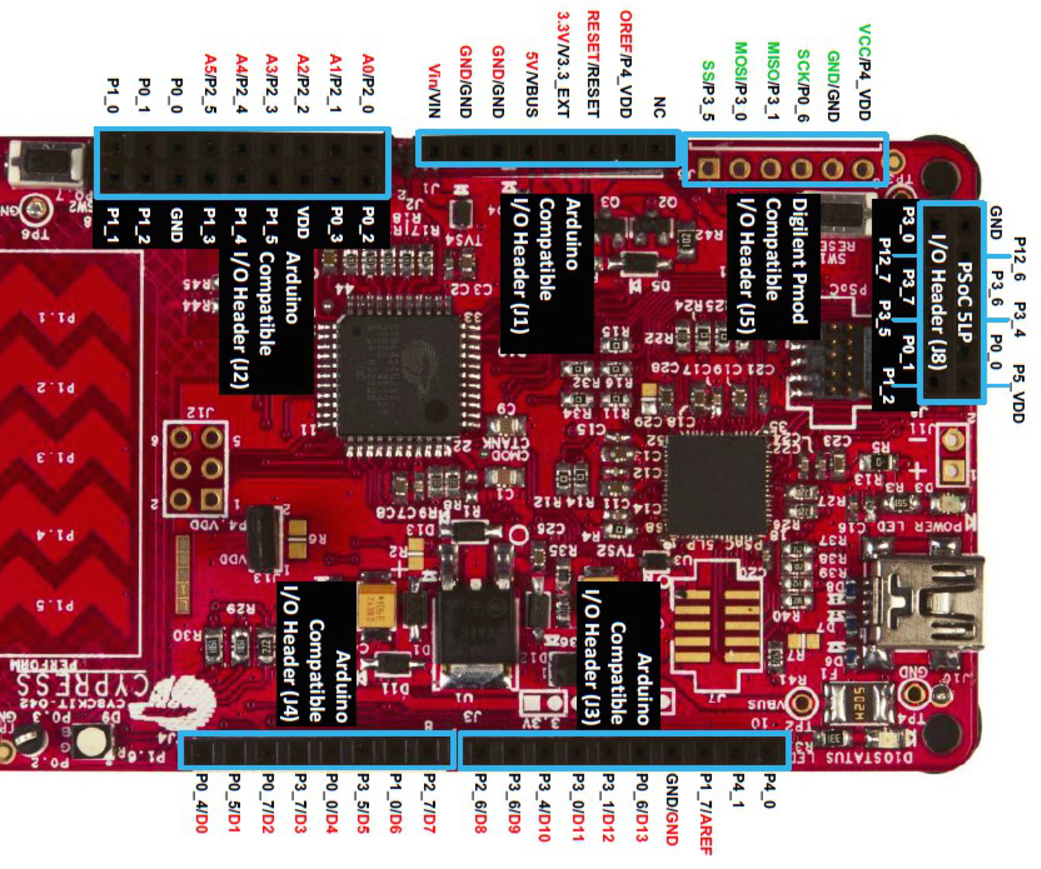
\includegraphics[width=0.7\textwidth]{filer/design/Billeder/psoc4_pin}}
\caption{Oversigt over fysiske pin-navne på PSoC4}
\label{lab:psoc4_pin}
\end{figure}

\newpage
\begin{table}[H]
\subsection{Master (HW)}
Her beskrives hvor mange og hvilke pins der skal benyttes på Devkit8000 til de forskellige forbindelser.
\caption{Tabel der viser pins på Devkit8000}
\begin{small}
\begin{tabular}{|p{3,5cm}|p{2cm}|p{2,9cm}|p{1,6cm}|p{2.6cm}|}
\hline

\textbf{Forbindelse}	&\textbf{Antal pins} 	&\textbf{Signalnavne} &\textbf{Pinnavne} &\textbf{Kommentar}  \\ \hline

SPI 	(P\_DK)			&5 						&MOSI				&J9.1		&					\\\cline{3-4}
					&						&MISO				&J9.2		&					\\\cline{3-4}
					&						&SCK					&J9.5		&					\\\cline{3-4}
					&						&SS0					&J9.3		&					\\\cline{3-4}					
					&						&GND					&J9.20		&					\\\hline

\end{tabular}
\end{small}
\label{table:master_forbindelse}
\end{table}

\begin{figure}[H]
\centering
{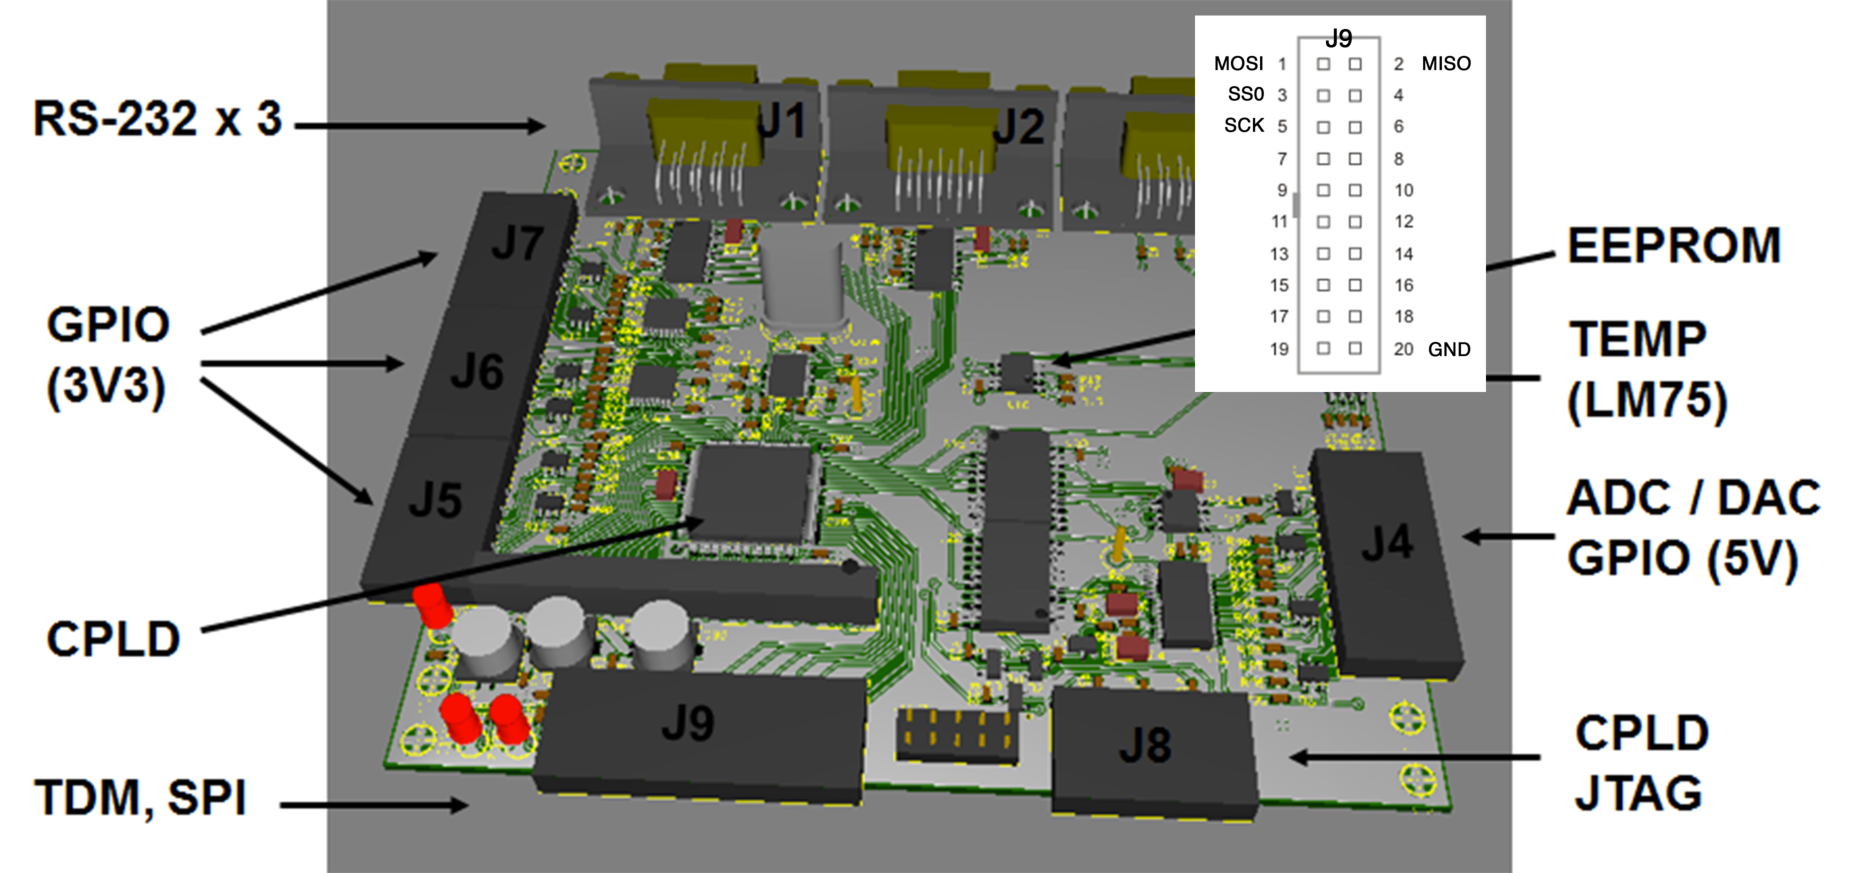
\includegraphics[width=\textwidth]{filer/design/Billeder/devkit_j9}}
\caption{Model af tilføjelses-print til Devkit8000 og J9-stik }
\label{lab:devkit_j9}
\end{figure}